 \documentclass{beamer}
\usepackage[latin1]{inputenc}
\usepackage{amsmath}
\usetheme{Warsaw}

\newcommand\applyFontA{\fontsize{6}{6}\selectfont}
\newcommand\applyFontB{\fontsize{8}{8}\selectfont}

\title[Credit Stress Testing]{Stress Testing of Migration Matrix and Loss Given Default}
\author{Michal Mackanic}
\institute{RMO/CZ}
\date{April 2018}

\begin{document}

\begin{frame}
	\titlepage
\end{frame}

\begin{frame}
	\frametitle{Outline}
	\tableofcontents[hideallsubsections]
\end{frame}

\AtBeginSection[]
{
  \begin{frame}<beamer>
    \frametitle{Section}
    \begin{beamercolorbox}[sep=4pt,center]{part title}
		\large{\insertsectionhead}\par%
    \end{beamercolorbox}
  \end{frame}
}

\AtBeginSubsection[]
{
  \begin{frame}<beamer>
    \frametitle{Section}
    \begin{beamercolorbox}[sep=4pt,center]{part title}
		\insertsubsectionhead\par%
    \end{beamercolorbox}
  \end{frame}
}

\AtBeginSubsubsection[]
{
  \begin{frame}<beamer>
    \frametitle{Section}
    \begin{beamercolorbox}[sep=2pt,center]{part title}
		\insertsubsubsectionhead\par%
    \end{beamercolorbox}
  \end{frame}
}

\applyFontB

\section{Symbols Used}

\begin{frame}{Symbols Used}
\begin{tabular}{l l}
$X_i$ & firm's log asset value\\
$\rho$ & correlation between asset returns and systematic risk factor\\
$Z$ & systematic risk factor\\
$z_t$ & value of systematic risk factor $Z$ at time period $t$\\
$\epsilon$ & idiosyncratic risk factor\\
$DR_i^t$ & default rate of rating group $i$ observed during time period $t$\\
$DR_i^{TTC}$ & average (aka through-the-cycle) observed default rate of rating group $i$\\
$PD_i$ & probability of default of rating group $i$\\
$PD_{TTC}$ & through-the-cycle probability of default\\
$PD_{stress}$ & stressed probability of default\\
$PM_{i,j}$ & probability of migrating from rating group $i$ to rating group $j$\\
$EL$ & expected loss\\
$loss_{stress}$ & stressed loss rate\\
$TH_{i,j}$ & threshold of rating group $i$ separating rating group $j-1$ and\\
 & rating group $j$\\
$n_i^t$ & counterparties within rating group $i$ during time period $t$\\
$k_{i,n}^t$ & defaults / migrations within rating group $i$ during\\
 & time period $t$\\
$M$ & number of macroeconomic variables included in regression model\\
$T$ & number of time periods used to determine $z_t$ and to estimate thresholds\\
$LM_{i,j}$ & maximum likelihood measure used to estimate threshold $TH_{i, j}$\\
$q$ & quantile of stressed probability of default\\
$k$ & LGD index risk\\
\end{tabular}
\end{frame}

\section{Stressing of Migration Matrix}

\begin{frame}{Introduction}
\setbeamertemplate{itemize items}[ball]
\begin{itemize}
	\item Consensus has been reached as most papers are based on Merton and Vasicek model.
	\item The proposed solution nicely fits into Basel framework.
	\item KBC credit guidelines introduced the same approach, which was subsequently applied in CSOB and K\&H.
	\item The main difference between current and proposed approach is that RMO suggests to stress the whole migration matrix rather than only vector of probability of defaults.
	\item RMO approach is based on "Stress-Testing Probability of Default and Migration Rate with respect to Basel II Requirements" by Peter Miu \& Bogie Ozdemir.
\end{itemize}
\end{frame}

\begin{frame}{The Model}
\setbeamertemplate{itemize items}[ball]
\begin{itemize}
	\item We assume that firm's log asset value is normally distributed (cornerstone of Merton / Vasicek model).
		\begin{equation}
			X = \sqrt{\rho} Z  + \sqrt{1 - \rho} \epsilon
		\end{equation}
	\item $Z \sim N[0, 1]$ represents systematic risk factor.
	\item $\epsilon \sim N[0, 1]$ represents idiosyncratic risk factor.
	\item $\rho$ represents correlation between systematic risk factor and asset returns. Value of $\rho$ is set up in line with Basel methodology.
\end{itemize}
\end{frame}

\begin{frame}{The Model}
\setbeamertemplate{itemize items}[ball]
\begin{itemize}
	\item A firm defaults if value of its assets falls under a certain threshold $TH_i$.
		\begin{multline}
			PD_i = P[X_i < TH_i] = P[\sqrt{\rho}Z + \sqrt{1 - \rho} 
			\epsilon_i < TH_i]=\\
			P\left[\epsilon_i < \frac{TH_i - \sqrt{\rho}Z}{\sqrt{1 - 
			\rho}}\right] = \Phi\left[\frac{TH_i - \sqrt{\rho}Z}{\sqrt{1 - 
			\rho}}\right].
		\end{multline}
	\item Similar approach could be used for migration probabilities.
		\begin{multline}
			PM_{i,j} = P[TH_{i, j + 1} \le X_i < TH_{i, j}] =\\
			P[TH_{i, j + 1} \le \sqrt{\rho}Z + \sqrt{1 - \rho} \epsilon_i < TH_{i, j}]=\\
			\Phi\left[\frac{TH_{i, j} - \sqrt{\rho}Z}{\sqrt{1 - 
			\rho}}\right] - \Phi\left[\frac{TH_{i, j + 1} - \sqrt{\rho}Z}{\sqrt{1 - 
			\rho}}\right].
		\end{multline}
\end{itemize}
\end{frame}

\begin{frame}{The Model}
\begin{figure}[htp]
\centering
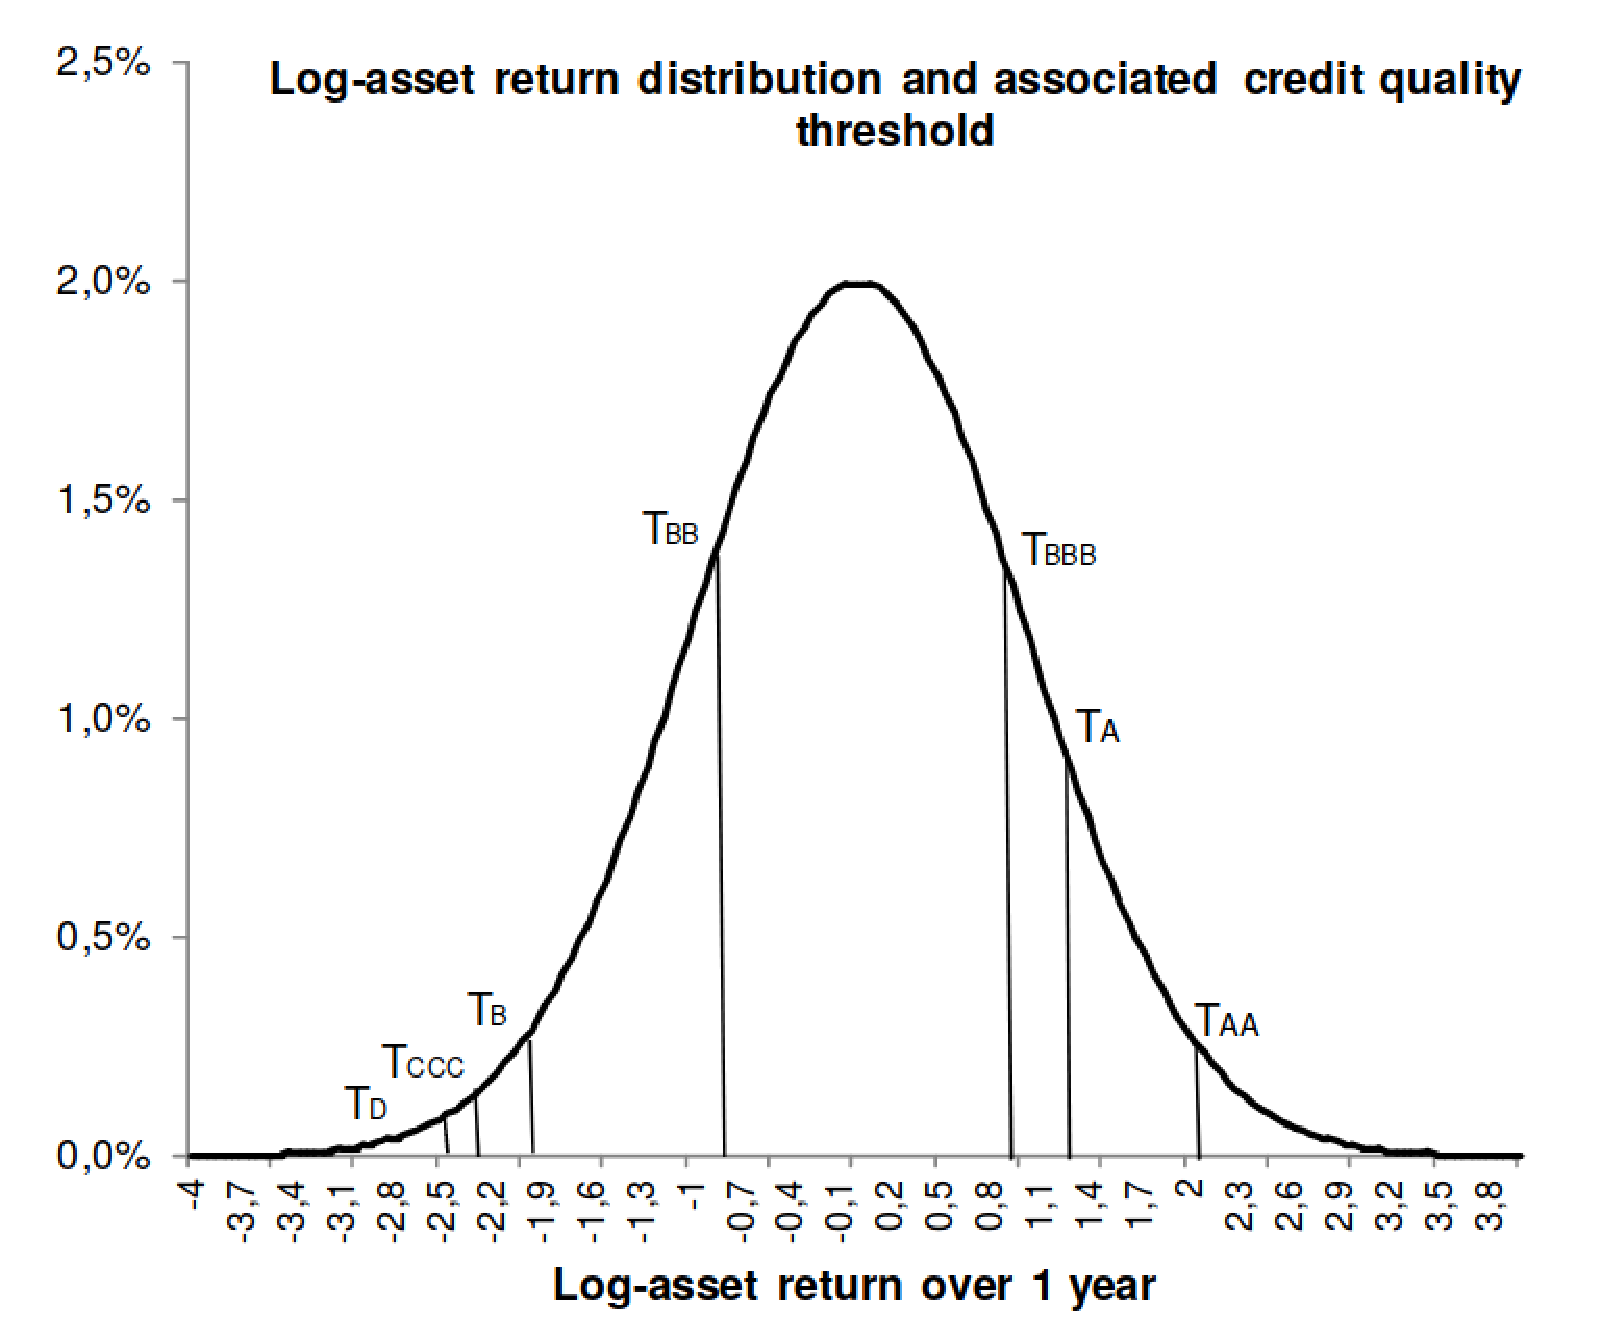
\includegraphics[scale = 0.25]{pictures/thresholds.eps}
\caption{Illustration of threshold concept}
\label{thresholds}
\end{figure}
\end{frame}

\begin{frame}{Systematic Risk}
\setbeamertemplate{itemize items}[ball]
\begin{itemize}
	\item Systematic risk factor $Z$ could be thought of as an economic cycle indicator.
		\begin{itemize}
			\item expansion year $\Rightarrow$ $z_t > 0$
			\item average year $\Rightarrow$ $z_t \approx 0$
			\item recession year $\Rightarrow$ $z_t < 0$
		\end{itemize}
	\item If we knew value $z_t$ of systematic risk factor $Z$, we could have calculated conditioned (aka stressed or point-in-time) probability of default.
		\begin{equation}
		PD_i = \Phi\left[\frac{TH_i - \sqrt{\rho}z_t}{\sqrt{1 - \rho}} | Z = 
		z_t\right].
		\end{equation}
\end{itemize}
\end{frame}

\begin{frame}{Systematic Risk}
\setbeamertemplate{itemize items}[ball]
\begin{itemize}
	\item However, we will go the other way around. Using observed default rates as proxy for conditioned probability of default and exploiting $TH_i = \Phi^{-1}(DR_i^{TTC})$, we determine $z_t$.
		\begin{equation}
			DR_i^t= \Phi\left[\frac{\Phi^{-1}[DR_i^{TTC}] - \sqrt{\rho}z_t}{\sqrt{1 - \rho}} | Z = z_t\right].
		\end{equation}
		\begin{equation}
			z_t = \frac{\Phi^{-1}[DR_i^{TTC}] - \Phi^{-1}[DR_i^t]\sqrt{1 - \rho}}{\sqrt{\rho}}.
		\end{equation}
	\item Please note that in theory default rate of any rating group could be used. However, since high ratings are less impacted by economic cycle, one should use default rates aggregated over lower ratings. Lower ratings are more sensitive to changes in economic cycle and therefore better in "extracting" information on level of systematic risk $Z$.
\end{itemize}
\end{frame}

\begin{frame}{Macroeconomic Variables}
\setbeamertemplate{itemize items}[ball]
\begin{itemize}
	\item Once we determine historical values $z_t$ of systematic risk factor $Z$, we can link them to macroeconomic variables via a regression model. Macroeconomic variables could be both current and lagged.
	\item Macroeconomic variables should be ideally normally distributed with zero mean and variance equal to one. Therefore one should try various transformations (log-odd, log ratio or log transformation) and standardize the result.
	\item Given the number of possible candidates, it is challenging to come up with an appropriate regression model.
	\item An example of a regression model is provided below.
		\begin{equation}
			z_t = \alpha + \beta_1 GDP_{t - 1} + \beta_2 IR^{5Y}_t + \beta_3 z_{t - 1} + \varepsilon_t
		\end{equation}
	\item When selecting macroeconomic variables into the model not only their statistical significance but also their importance for stress scenario formulation should be considered.
\end{itemize}
\end{frame}

\begin{frame}{Threshold Calibration}
\setbeamertemplate{itemize items}[ball]
\begin{itemize}
	\item Conditioned (aka stressed or point-in-time) migration matrix is defined through
		\begin{equation}
			PM_{i,j} = \Phi\left[\frac{TH_{i, j} - \sqrt{\rho}Z}{\sqrt{1 - 
			\rho}}\right] - \Phi\left[\frac{TH_{i, j + 1} - \sqrt{\rho}Z}{\sqrt{1 - 
			\rho}}\right].
		\end{equation}
	\item Remember we know $z_t$ and $\rho$. Therefore we have to estimate threshold $TH_{i, j}$.
	\item Please note that the thresholds are not function of time, i.e. they do not change with economic cycle.
	\item We estimate the thresholds using maximum likelihood so that for given $z_t$ and $\rho$ they imply historical point-in-time migration matrices which match observed migrations / defaults as close as possible.
\end{itemize}
\end{frame}

\begin{frame}{Threshold Calibration}
\setbeamertemplate{itemize items}[ball]
\begin{itemize}
	\item Consider a migration matrix with $N$ rating groups and let us focus on a general rating group $i$.
	\item In theory we are to estimate $N + 1$ thresholds. However, the first threshold $TH_{i,1}$ and the last threshold $TH_{i, N + 1}$ are not estimated as they are by definition equal to $\infty$ and $-\infty$ respectively. That leaves us with $N - 1$ thresholds to estimate.
	\item Let us focus at time period  $t$. Assume that the rating group consists of $n_i^t$ counterparties and that we observe $k_{i, j}^t$ migrations / defaults. Then (for a given threshold) probability of this event is
		\begin{equation}
			p_{i, N}^t = \binom{n_i^t}{k_{i, j}^t} \left(PM_{i,j}^t\right)^{k_{i, 
			j}^t} \left(1 - PM_{i,j}^t\right)^{n_i^t - k_{i, j}^t}.
		\end{equation}
	\item To find an optimal threshold $TH_{i, j}$ we have to maximize probabilities across all time periods, i.e. we maximize $LM_{i, j} = \sum_{t = 1}^T \log(p_{i, j}^t)$ by changing value of threshold $TH_{i,j}$.
	\item Optimal value of threshold $TH_{i, j}$ could be easily found using a grid search method.
	\item Optimization process starts with default state and continues towards the best rating.
	\item In this way we estimate all thresholds one by one for all rating groups.
\end{itemize}
\end{frame}

\begin{frame}{Link Between PIT and TTC}
\setbeamertemplate{itemize items}[ball]
\begin{itemize}
	\item PIT migration matrix could be thought of as a migration matrix conditioned on state of an economic cycle.
	\item TTC migration matrix could be thought of as a migration matrix over the whole economic cycle.
	\item Please note that state of economic cycle is indicated by value $z_t$ of systematic risk factor $Z$.
	\item Migration matrix is fully determined by $z_t$, $\rho$ and thresholds.
	\item Since $z_{TTC} \approx 0$, the estimated thresholds define not only PIT but also TTC migration matrix.
	\item Therefore the above procedure enables us to estimate consistent PIT and TTC migration matrices.
\end{itemize}
\end{frame}

\begin{frame}{Stress Testing}
\setbeamertemplate{itemize items}[ball]
\begin{enumerate}
	\item Split historical data in several non-overlapping time periods $t = 1, 2, ..., T$. 
	The periods typically represent quarters, half-years or years.
	\item Determine number of observed migrations and defaults per rating group for each time period $t = 1, 2, ..., T$.
	\item Using data from the previous step, determine aggregated default rates 
	for non-investment rating groups for each time period $t = 1, 2, ..., T$.
	\item Fix value of correlation $\rho$ in line with Basel methodology.
	\item Using default rates from step (3) determine values $z_t$ 
	of systematic risk factor $Z$ for each time period $t = 1, 2, ..., T$.
	\item Construct an appropriate regression model that establishes a 
	link between systematic risk factor $Z$ and macroeconomic variables.
	\item Using observed defaults and migrations during time periods $t = 1, 2, ..., T$ calibrate thresholds, which define historical point-in-time 
	migration matrices and consistent through-the-cycle migration matrix (which could be for example determined via $z_{TTC} = 0$).
	\item Take stressed macroeconomic variables and determine corresponding 
	value $z_{stress}$ of systematic risk factor $Z$ using regression model 
	introduced in step (6).
	\item Using $z_{stress}$ and thresholds calibrated in step (7) 
	construct point-in-time migration matrix that corresponds to stressed 
	macroeconomic variables.
\end{enumerate}
\end{frame}

\section{Stress Testing LGD}

\begin{frame}{Introduction}
\setbeamertemplate{itemize items}[ball]
\begin{itemize}
	\item Consensus has not been reached as several papers are introducing different approaches to the problem.
	\item RMO approach follows "Loss given default as a function of the default rate" by Jon Frye as we found his approach as the most pragmatic and
	since it naturally fits into concept of stressing migration matrix.
\end{itemize}
\end{frame}

\begin{frame}{The Model}
\setbeamertemplate{itemize items}[ball]
\begin{itemize}
	\item The main idea is that LGD is increasing with increasing probability of default, i.e. LGD and probability of default are comonotonic.
	\item This means that LGD quantiles map directly to quantiles of probability of default, e.g. 20\% LGD quantile corresponds to 20\% quantile of probability of default.
	\item Therefore, if we knew quantile of a stressed probability of default, we could use the quantile to determine corresponding stressed LGD.
	\item Let us assume that through-the-cycle probability of default is known. Using Vasicek model, quantile of a stressed probability of default is
		\begin{equation}
			q = \Phi \left[\frac{\sqrt{1 - \rho} \Phi^{-1}[PD_{stress}] - 
			\Phi^{-1}[PD_{TTC}]}{\sqrt{\rho}}\right].
		\end{equation}
	\item Suppose that stressed loss rate also obeys Vasicek distribution. Using the above derived quantile $q$ and expected loss $EL$, the stressed loss rate is defined by
		\begin{equation}
			loss_{stress} = \Phi\left[\Phi^{-1}[PD_{stress}] - \frac{\Phi^{-1}[PD_{TTC}] - \Phi^{-1}[EL]}{\sqrt{1 - \rho}}\right].
		\end{equation}
\end{itemize}
\end{frame}

\begin{frame}{The Model}
\setbeamertemplate{itemize items}[ball]
\begin{itemize}
	\item Stressed LGD could be easily calculated as a ratio of stressed loss rate and stressed probability of default
		\begin{equation}
			LGD_{stress} = \frac{loss_{stress}}{PD_{stress}} = \frac{\Phi\left[\Phi^{-1}[PD_{stress}] - 
			k\right]}{PD_{stress}}
		\end{equation}
		where
		\begin{equation}
			k = \frac{\Phi^{-1}[PD_{TTC}] - \Phi^{-1}[EL]}{\sqrt{1 - \rho}}
		\end{equation}
		is called LGD risk index and which fully determines LGD function.
\end{itemize}
\end{frame}

\begin{frame}{The Model}
\begin{figure}[htp]
\centering
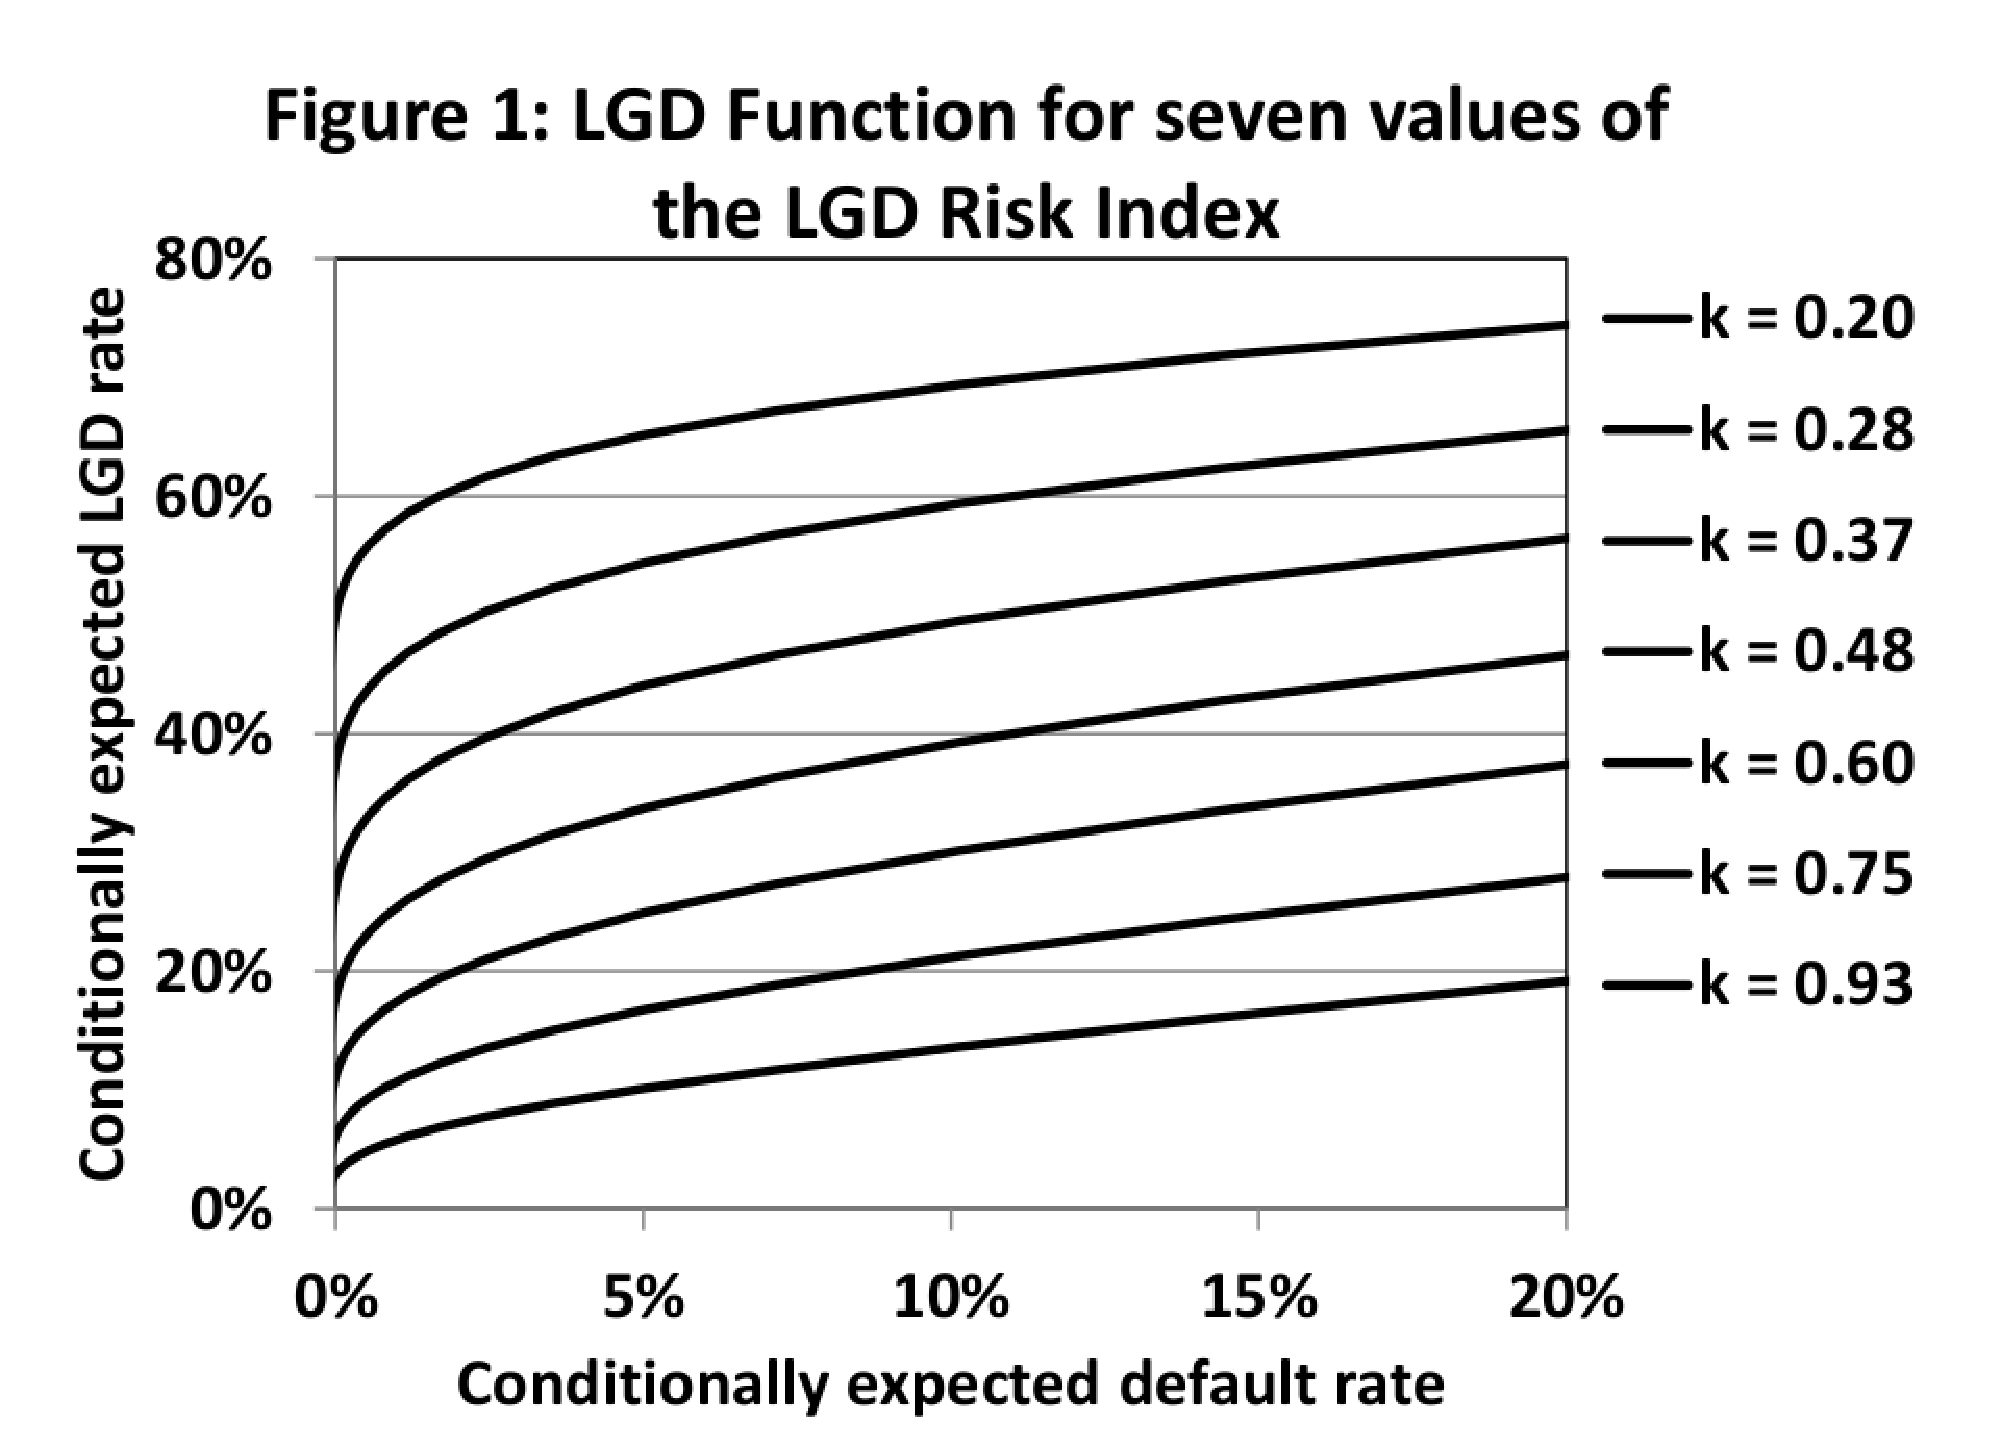
\includegraphics[scale = 0.20]{pictures/lgd-function.eps}
\caption{LGD function for different levels of $k$}
\label{lgd-function}
\end{figure}
\end{frame}

\begin{frame}{The Model}
\setbeamertemplate{itemize items}[ball]
\begin{itemize}
	\item Advantages
		\begin{itemize}
			\item LGD function is very easy to calibrate.
			\item The model fits into concept of migrating matrix stressing.
		\end{itemize}
	\item Disadvantages
		\begin{itemize}
			\item Loss rates is assumed to follow Vasicek distribution. However, no sound economic explanation is provided.
			\item The model is tested on US corporate bonds. There is no guarantee it will work on retail portfolios as well.
			\item Loss rate function is fully determined by expected loss. This means one can only change level but not shape of LGD curve; for illustration see figure on the previous slide.
		\end{itemize}
\end{itemize}
\end{frame}

\begin{frame}{The Model}
\setbeamertemplate{itemize items}[ball]
\begin{itemize}
	\item Comonotonicity of LGD and probability of default could be easily used to introduce other probability distributions.
	\item We replaced Vasicek distribution with beta distribution. The distribution could be fitted to LGDs historically observed through out economic cycle
	or calibrated on expert opinion.
	\item Given quantile implied by stressed probability of default, we use the quantile to sample from beta distribution to get a consistenly stressed LGD.
	\item Beta distribution could be set up in a way that it matches LGD function based on Vasicek distribution. Besides it is more flexible in terms of possible shapes.
\end{itemize}
\end{frame}

\begin{frame}{The Model}
\begin{figure}[htp]
\centering
\includegraphics[scale = 0.20]{pictures/lgd-test.eps}
\caption{LGD function based on Vasicek and beta distribution}
\label{lgd-test}
\end{figure}
\end{frame}

\begin{frame}{Mortgage Portfolio}
\setbeamertemplate{itemize items}[ball]
\begin{itemize}
	\item Concept introduced in "Stress Testing the Credit Risk of Mortgage Loans:
	The Relationship between Portfolio-LGD and the Loan-to-Value Distribution" by Christian Greve and Lutz Hahnenstein could by applied to mortgage (and other collateralized) portfolios.
	\item The main idea is that LGD is fully determined by actual value of loan collateral. Therefore LGD of a mortgage loan is driven by its loan-to-value and real-estate shocks.
	\item To apply the concept on portfolio level, it is assumed that portfolio's loan-to-value composition could be described via beta distribution
	and that LGD for a given loan-to-value $X$ and recovery rate $rr$ is $1 - \frac{rr}{\max[X, rr]}$.
	\item It can be proved that under these assumptions average portfolio LGD is
		\begin{equation}
			E[LGD] = 1 - F^{\alpha, \beta}(rr) - rr \frac{\alpha + \beta - 1}{\alpha - 1}(1 - F^{\alpha - 1, \beta}(rr)),
		\end{equation}
	where $F^{\alpha, \beta}$ is cumulative distribution of beta distribution with parameters $\alpha$ and $\beta$.
\end{itemize}
\end{frame}

\begin{frame}{Mortgage Portfolio}
\setbeamertemplate{itemize items}[ball]
\begin{itemize}
	\item We expressed mean portfolio LGD as a function of the mean recovery rate $rr$ and of the two parameters $\alpha$ and $\beta$
	that capture the portfolio's loan-to-value distribution.
	\item Please note portfolio LGD is stressed through stressing average recovery rate $rr$ rather than through stressing current loan-to-value.
	\item As illustrated on next slide, two portfolios with the same average loan-to-value could have quite different average LGD; check portfolios' LGD for a real estate shock of -30\%.{}
	General rule is that portfolios with more widespread distribution of loan-to-values tend to have larger average LGD.
\end{itemize}
\end{frame}

\begin{frame}{Mortgage Portfolio}
\begin{figure}[htp]
\centering
\includegraphics[scale = 0.20]{pictures/lgd-mortgages.eps}
\caption{Loan-to-value based LGD as a function of a real estate price shock}
\label{lgd-mortgages}
\end{figure}
\end{frame}

\begin{frame}{Mortgage Portfolio}
\setbeamertemplate{itemize items}[ball]
\begin{itemize}
	\item Advantages
	\begin{itemize}
		\item The model is intuitive and easy to understand.
		\item Beta function describing portfolio's composition of loan-to-value could be easily calibrated on real data; no expert input is needed.
	\end{itemize}
	\item Disadvanges
		\begin{itemize}
			\item Only secured recoveries are considered.
			\item LGD is stressed only via real estate shocks. Other potentially import macroeconomic variables are ignored.
		\end{itemize}
\end{itemize}
\end{frame}

\end{document}
